\documentclass[12pt
,headinclude
,headsepline
,bibtotocnumbered
]{scrartcl}
\usepackage[paper=a4paper,left=25mm,right=25mm,top=25mm,bottom=25mm]{geometry} 
\usepackage[utf8]{inputenc}
\usepackage[ngerman]{babel}
\usepackage{graphicx}
\usepackage{multirow}
\usepackage{pdfpages}
%\usepackage{wrapfig}
\usepackage{placeins}
\usepackage{float}
\usepackage{flafter}
\usepackage{mathtools}
\usepackage{hyperref}
\usepackage{epstopdf}
\usepackage[miktex]{gnuplottex}
\usepackage[T1]{fontenc}
\usepackage{mhchem}
\usepackage{fancyhdr}
%\setlength{\mathindent}{0pt}
\usepackage{amssymb}
\usepackage[list=true, font=large, labelfont=bf, 
labelformat=brace, position=top]{subcaption}
\setlength{\parindent}{0mm}

\setlength{\parindent}{0mm}

\pagestyle{fancy}
\fancyhf{}
\lhead{Physikalische Geodäsie\\Übung 5: Gravitation (Teil 3)}
\rhead{Hsin-Feng Ho \\3378849}
\rfoot{Seite \thepage}
\begin{document}
	\begin{titlepage}
		\vspace{\fill}
		\title{\textbf{Physikalische Geodäsie \\ Übung 5: Gravitation (Teil 3)}}
		\vspace{5cm}
		\author{Hsin-Feng Ho\\
			3378849}
		\vspace{3cm}
		\maketitle
	\end{titlepage}
\section{Grafische Darstellung der Messwerte}
Eine fiktive gravimetischen Messkampagne entlang eines Profils wurde durchgeführt. In dieser Aufgabe sind die Messwerte graphisch darzustellen.
\begin{figure}[H]
	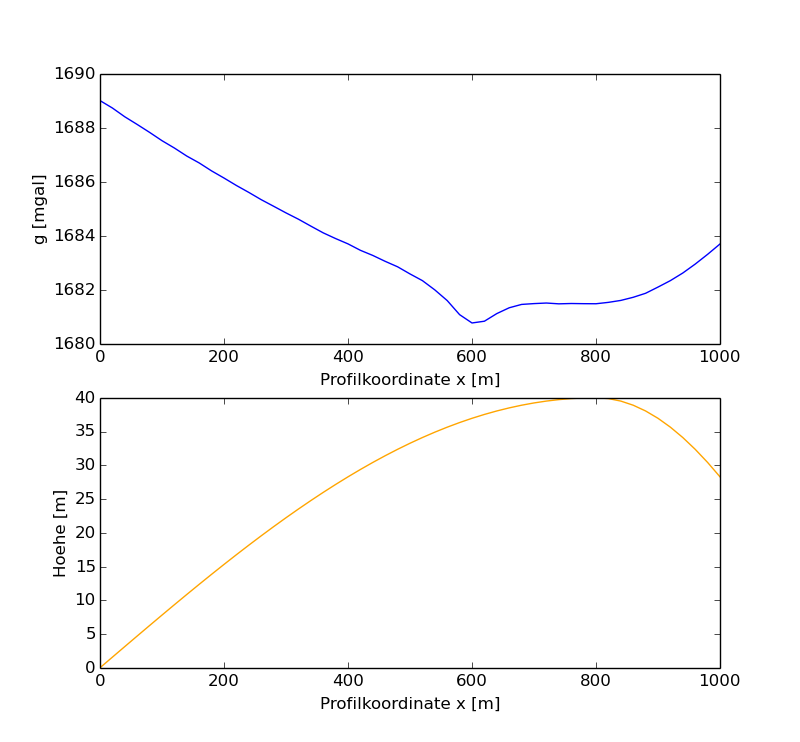
\includegraphics[width=15cm]{figure_1}
	\caption{Schwere und Höhe in Abhänigkeit von Profilkoordinaten}
\end{figure}
Es ist deutlich zu erkennen, dass die Kurve von Schwere an der Stelle von etwa 600 m plötzlich eingefallen ist.
\section{Korrektur der Höhe}
Da die Messwerte der Schwere von den unterschiedlichen Höhen abhängen, sind die Messwerte zu korrigieren.
\begin{itemize}
	\item Freiluft-Korrektur=$-0,3\frac{mgal}{m}\cdot h$
	\item Bouguer-Korrektur=$2\pi G \rho h=0,1119\frac{mgal}{m}\cdot h$
\end{itemize}
\begin{figure}[H]
	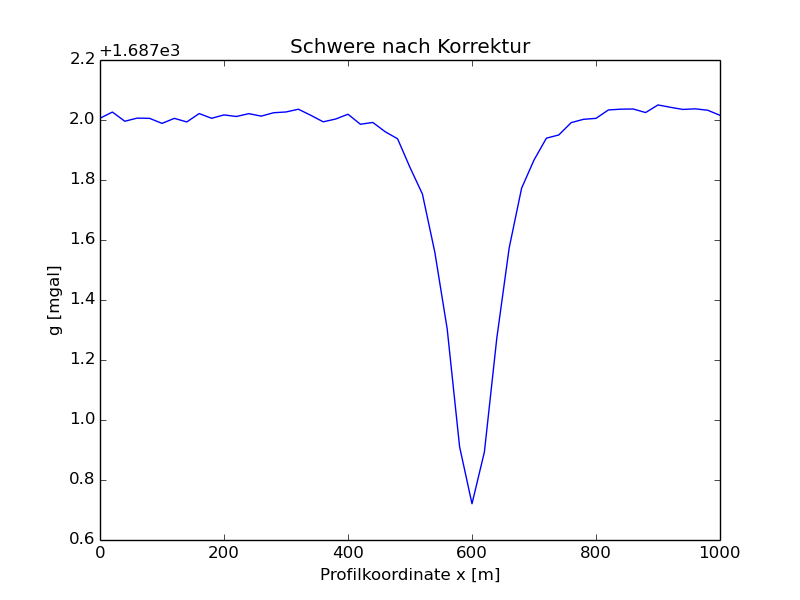
\includegraphics[width=15cm]{figure_2}
\end{figure}
Aus der Graphik vermuten wir, dass die Profikoordinate X der Höhle 600m ist.
\section{Schwerestörung}
Nun wird eine Funktion implementiert, damit der vertikale Anteil der Schwerestörung $\boldsymbol{g}_z(x)$ bestimmt werden kann.
\begin{align*}
	|a|&=-\frac{4}{3}\pi G\rho R^3\frac{1}{r^2}\\
	r&=\sqrt{(X-x)^2+(z+R)^2}\\
	a_z&=|a|\sin(\frac{Z+R}{r})
\end{align*}
\section{Modellieren der Schwerestörung}
Aus der Ergebnisse der Aufgabe 2 können wir feststellen, dass die Störung ungefähr $\boldsymbol{g}_z(x)=1,28\,\mathrm{mgal}$ beträgt.
\\ \\
Mit den Werte $Z=500\,\mathrm{m}, R=1890\,\mathrm{m}$ ergibt sich $\boldsymbol{g}_z(x)=1,28\,\mathrm{mgal}$. Da mit anderen Kombinationen sehr schwer an der Nähe vom Wert kommen, würde ich sagen, dass das Ergebnis eindeutig ist.
\section{Bestimmung ohne Dichte}
Vergleich der Schwerestörungen $\boldsymbol{g}_z(x)$ mit $\rho_1=2700, \rho_2=1000$
\begin{align*}
	\boldsymbol{g}_{z1}=1.28\,\mathrm{mgal}\\
	\boldsymbol{g}_{z2}=1.30\,\mathrm{mgal}
\end{align*}
Da die Schwerestörung nur wenig mit sehr unterschiedlichen Dichten abweicht, ist Radius R und Tiefe Z der Höhe eindeutig bestimmbar trotz unbekannter Dichte.
\end{document}